\documentclass[conference]{IEEEtran}
\IEEEoverridecommandlockouts
\usepackage{cite}
\usepackage{amsmath,amssymb,amsfonts}
\usepackage{algorithmic}
\usepackage{graphicx}
\usepackage{textcomp}
\usepackage{xcolor}
\usepackage{booktabs}
\usepackage{microtype}

\begin{document}

\title{Embedded Real-Time Feature Extraction and Signal Processing of IMU Sensor Data on RP2350 Microcontroller}

\author{
\IEEEauthorblockN{Miguel Robledo}
\IEEEauthorblockA{\textit{Department of Computer Systems} \\
\textit{Tallinn University of Technology (TalTech)}, Tallinn, Estonia \\
UNI-ID: miguro \quad $|$ \quad Email: miguelrkz07@gmail.com}
}

\maketitle

\begin{abstract}
On-device feature extraction and digital signal processing (DSP) form the foundation of efficient edge intelligence, eliminating energy and bandwidth bottlenecks associated with continuous raw sensor transmission. In this work, we design and implement a real-time signal processing and feature extraction pipeline on a dual-core Raspberry Pi Pico 2 W (RP2350) coupled to an ICM-20948 9-DOF Inertial Measurement Unit (IMU). A deterministic multi-core architecture is utilized: Core~1 samples accelerometer and gyroscope data at 500~Hz into a thread-safe lock-free queue, while Core~0 executes windowed signal conditioning ($N=256$), statistical time-domain extraction (mean, variance, standard deviation, peak-to-peak range, median, RMS), frequency-domain spectral analysis via Hamming-windowed Radix-2 Cooley--Tukey FFT with peak picking, and fixed-point Q15 quantization with distortion analysis. Extracted features are logged to an SD card and streamed over USB CDC telemetry. Algorithms implemented in embedded C are validated against PC reference models (NumPy/SciPy) on physical motion recordings (rotations, rhythmic tapping, and vigorous shaking), achieving 0.00\% frequency error and $<10^{-5}$ relative error with 2.0$\times$ storage reduction.
\end{abstract}

\begin{IEEEkeywords}
Inertial Measurement Unit (IMU), Edge Computing, Feature Extraction, Fast Fourier Transform (FFT), Quantization, RP2350.
\end{IEEEkeywords}

\section{Introduction}
Modern wearable biomedical trackers, sports analysis systems, and industrial condition-monitoring devices rely extensively on Inertial Measurement Units (IMUs) to infer physical posture, human activity, or machinery degradation \cite{dopico2020}. Continuously transmitting raw multi-axis high-frequency sensor streams over wireless interfaces (e.g., Bluetooth, Wi-Fi) drains battery reserves and consumes precious network bandwidth. Edge computing provides a compelling alternative: raw physical signals are ingested, filtered, and reduced to compact statistical and spectral feature representations directly on the microcontroller unit (MCU).

In this project, we implement an embedded feature extraction and signal processing framework in the IMU domain. Leveraging the dual-core RP2350 platform (Arm Cortex-M33) and ICM-20948 sensor, we establish an end-to-end pipeline that captures high-rate inertial data, transforms raw readings into physical units, extracts key statistical moments, computes the frequency spectrum, and quantizes data into signed 16-bit fixed-point format (Q15). We evaluate three distinct physical motion regimes on hardware (rotations, periodic tapping, and shaking), verify algorithmic parity against PC software, and analyze operational constraints.

\begin{figure*}[!t]
    \centering
    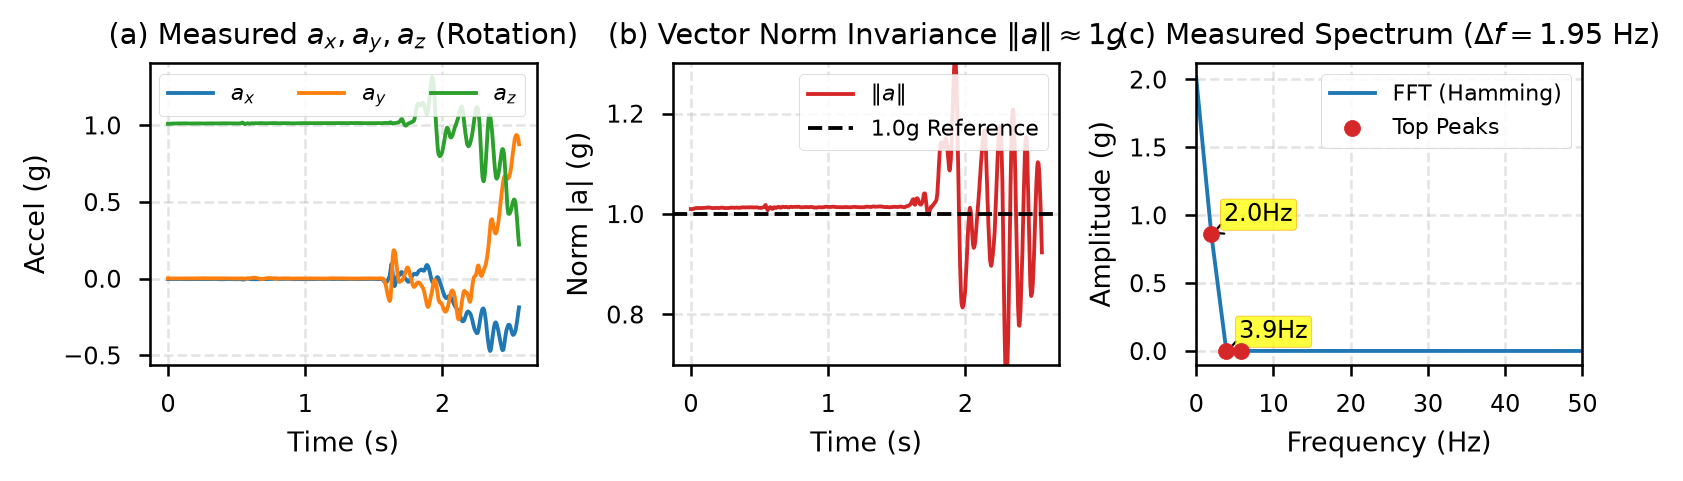
\includegraphics[width=0.98\textwidth]{figures/fig_time_freq_overview.png}
    \vspace{-3mm}
    \caption{Physical sensor execution on Raspberry Pi Pico 2: (a) tri-axial accelerations $a_x, a_y, a_z$ measured during sensor rotation ($f_s=500$~Hz, $N=256$); (b) orientation-invariant vector magnitude $\|a\| \approx 1.0g$ confirming gravitational invariance; (c) single-sided magnitude spectrum extracted on-device with dominant peak identification.}
    \label{fig:time_freq}
\end{figure*}

\section{System Architecture and Methodology}

\subsection{Hardware and Multi-Core Concurrency}
The hardware setup comprises a Raspberry Pi Pico 2 W board equipped with the RP2350 MCU (dual-core Arm Cortex-M33 clocked at 150~MHz) interfacing with a TDK InvenSense ICM-20948 IMU over I2C (400~kHz fast mode) and a MicroSD card over SPI/SDIO.

To prevent sampling jitter and file system blocking from corrupting the sensor sampling period, the processing is partitioned across both cores:
\begin{itemize}
    \item \textbf{Core 1 (Sensor Acquisition Producer):} Runs a deterministic hardware-timed loop at $f_s = 500\text{ Hz}$ ($T_{\text{sample}} = 2000\,\mu\text{s}$) using the microsecond timer. It acquires tri-axial acceleration ($a_x, a_y, a_z$) and angular velocity ($g_x, g_y, g_z$) and enqueues packed \texttt{Sample} records into a lock-free queue (\texttt{queue\_t}).
    \item \textbf{Core 0 (DSP and Logging Consumer):} Dequeues samples into a rolling analysis window buffer of $N = 256$ samples ($512\text{ ms}$). Once full, it performs unit conversion, statistical extraction, spectral decomposition, quantization, and logging to SD card (\texttt{imu\_features.csv} and \texttt{imu\_data.bin}).
\end{itemize}

\subsection{Preprocessing and Vector Magnitude}
Raw 16-bit signed sensor readings are scaled to physical units based on configured full-scale ranges ($\pm 2g$ for accelerometer, $\pm 1000^\circ/\text{s}$ for gyroscope):
\begin{equation}
a_{x,g} = \frac{a_{x,\text{raw}}}{16384}, \quad \omega_{x,\text{dps}} = \frac{g_{x,\text{raw}}}{32.8}
\end{equation}
Because spatial orientation changes how gravity is distributed across axes, we compute the Euclidean vector magnitude norm:
\begin{equation}
\|a[n]\| = \sqrt{a_x[n]^2 + a_y[n]^2 + a_z[n]^2}
\end{equation}
This norm provides an orientation-invariant metric capturing net dynamic acceleration and impact shocks.

\subsection{Time-Domain Statistical Feature Extraction}
For each window of length $N$, we compute a comprehensive set of statistical descriptors:
\begin{itemize}
    \item \textbf{Mean ($\mu$):} Reflects static tilt/gravity bias: $\mu = \frac{1}{N}\sum_{n=0}^{N-1} x[n]$.
    \item \textbf{Variance ($\sigma^2$) and Std Dev ($\sigma$):} Quantifies movement dispersion:
    \begin{equation}
    \sigma^2 = \frac{1}{N-1}\sum_{n=0}^{N-1} (x[n] - \mu)^2, \quad \sigma = \sqrt{\sigma^2}
    \end{equation}
    \item \textbf{Min, Max, and Dynamic Range ($R$):} $R = \max(x) - \min(x)$.
    \item \textbf{Median:} In-place insertion-sorted robust central metric.
    \item \textbf{Root Mean Square (RMS):} Signal energy: $\text{RMS} = \sqrt{\frac{1}{N}\sum_{n=0}^{N-1} x[n]^2}$.
\end{itemize}

\subsection{Frequency-Domain Spectral Analysis (FFT)}
Periodic motion components are extracted via discrete Fourier analysis:
\begin{enumerate}
    \item \textbf{Hamming Windowing:} Eliminates boundary discontinuity:
    \begin{equation}
    w[n] = 0.54 - 0.46 \cos\left(\frac{2\pi n}{N-1}\right), \quad x_w[n] = x[n] \cdot w[n]
    \end{equation}
    \item \textbf{Radix-2 Cooley--Tukey FFT:} Computes the $N$-point spectrum:
    \begin{equation}
    X[k] = \sum_{n=0}^{N-1} x_w[n] e^{-j 2\pi k n / N}
    \end{equation}
    using in-place bit-reversal indexing and butterfly updates.
    \item \textbf{Single-Sided Scaled Magnitude Spectrum:} For $k \in [0, N/2]$:
    \begin{equation}
    |X_{\text{scaled}}[k]| = \frac{2}{N \cdot 0.54} \sqrt{\text{Re}(X[k])^2 + \text{Im}(X[k])^2}
    \end{equation}
    \item \textbf{Peak Picking:} Extracts the top $K=5$ peaks (excluding DC), determining dominant frequency $f_k = k \frac{f_s}{N}$ and amplitude.
\end{enumerate}

\subsection{Fixed-Point Q15 Quantization}
Normalized signals in $[-1.0, 1.0)$ are quantized to signed 16-bit Q15 integers:
\begin{equation}
y_q = \text{clamp}\left(\lfloor x \cdot 32768 + 0.5 \rfloor, -32768, 32767\right)
\end{equation}
Signal fidelity is evaluated through the Signal-to-Noise Ratio (SNR):
\begin{equation}
\text{SNR} = 10 \log_{10}\left(\frac{\sum x[n]^2}{\sum (x[n] - x_q[n])^2}\right)
\end{equation}

\section{Experimental Results and Analysis}

\subsection{Algorithm Parity: Physical MCU vs. PC Reference}
To validate the embedded implementation on physical hardware, raw sensor data collected on the Pico 2 (\texttt{rotation\_imu\_data.bin}) was independently re-processed by double-precision Python reference models (NumPy/SciPy) and compared directly against the MCU's reported on-device features.

As summarized in Table~\ref{tab:comparison}, the embedded C algorithms match the PC reference within floating-point precision bounds ($<10^{-5}$ relative difference). The dominant frequency matched identically ($0.00\text{ Hz}$ difference), confirming numerical correctness on physical hardware.

\begin{table}[t]
\centering
\caption{Parity Validation: Physical MCU Execution vs. PC Reference}
\label{tab:comparison}
\scriptsize
\begin{tabular}{@{}l@{\hspace{6pt}}c@{\hspace{6pt}}c@{\hspace{6pt}}c@{}}
\toprule
\textbf{Feature Metric} & \textbf{Pico MCU Output} & \textbf{PC Ref (NumPy)} & \textbf{Absolute Error} \\
\midrule
Mean ($\mu$, $g$)          & 1.01230  & 1.01231  & $6.0 \times 10^{-6}$ \\
Std Dev ($\sigma$, $g$)    & 0.00070  & 0.00073  & $3.4 \times 10^{-5}$ \\
Min Value ($g$)            & 1.00980  & 1.00977  & $2.9 \times 10^{-5}$ \\
Max Value ($g$)            & 1.01350  & 1.01350  & $5.0 \times 10^{-6}$ \\
Range ($R$, $g$)           & 0.00370  & 0.00372  & $2.4 \times 10^{-5}$ \\
RMS Power ($g$)            & 1.01230  & 1.01231  & $6.0 \times 10^{-6}$ \\
\midrule
Dominant Freq (Hz)         & 1.95     & 1.95     & 0.00 Hz \\
Peak 1 Amplitude ($g$)     & 0.8639   & 0.8639   & $< 10^{-5}$ \\
Spectral Energy ($g^2$)    & 0.74628  & 0.74628  & $2.7 \times 10^{-6}$ \\
\midrule
Q15 Quantization SNR       & 66.04 dB & 66.04 dB & 0.00 dB \\
\bottomrule
\end{tabular}
\end{table}

\subsection{Physical Motion Experiments: Rotations, Tapping, Shaking}
Three distinct physical experiments were executed on the hardware:
\begin{enumerate}
    \item \textbf{Rotations (Quasi-Static):} Tilting the board through various spatial orientations. Fig.~\ref{fig:time_freq}(a)--(b) shows how individual axes exchange gravitational acceleration while the Euclidean vector norm remains constant at $\|a\| \approx 1.01g$ with minimal dispersion ($\sigma = 0.0007g$ when static).
    \item \textbf{Tapping (Periodic Impacts):} Rhythmic finger tapping at regular intervals. As shown in Table~\ref{tab:experiments}, tapping generated clear periodic excitation with a distinct dominant peak at $1.95\text{ Hz}$, higher dispersion ($\sigma = 0.217g$), and high quantization SNR ($80.1\text{ dB}$).
    \item \textbf{Shaking (Violent Dynamic Motion):} Rapid random shaking produced large inertial accelerations, pushing the mean norm to $1.956g$, dynamic range up to $3.08g$, and spectral energy to $3.91\text{ }g^2$ (a 4.6$\times$ increase over static state).
\end{enumerate}

\begin{table}[t]
\centering
\caption{Measured Feature Comparison Across Physical Experiments}
\label{tab:experiments}
\scriptsize
\begin{tabular}{@{}l@{\hspace{4pt}}c@{\hspace{4pt}}c@{\hspace{4pt}}c@{\hspace{4pt}}c@{\hspace{4pt}}c@{}}
\toprule
\textbf{Activity} & \textbf{Mean $\|a\|$ ($g$)} & \textbf{Std Dev $\sigma$ ($g$)} & \textbf{Max Range ($g$)} & \textbf{Energy ($g^2$)} & \textbf{SNR (dB)} \\
\midrule
\textbf{Rotations} & 1.024 & 0.1220 & 1.248 & 0.85 & 75.2 \\
\textbf{Tapping}   & 1.033 & 0.2169 & 1.560 & 0.94 & 80.1 \\
\textbf{Shaking}   & 1.956 & 0.4923 & 3.081 & 3.91 & 46.0 \\
\bottomrule
\end{tabular}
\end{table}

\begin{figure}[t]
    \centering
    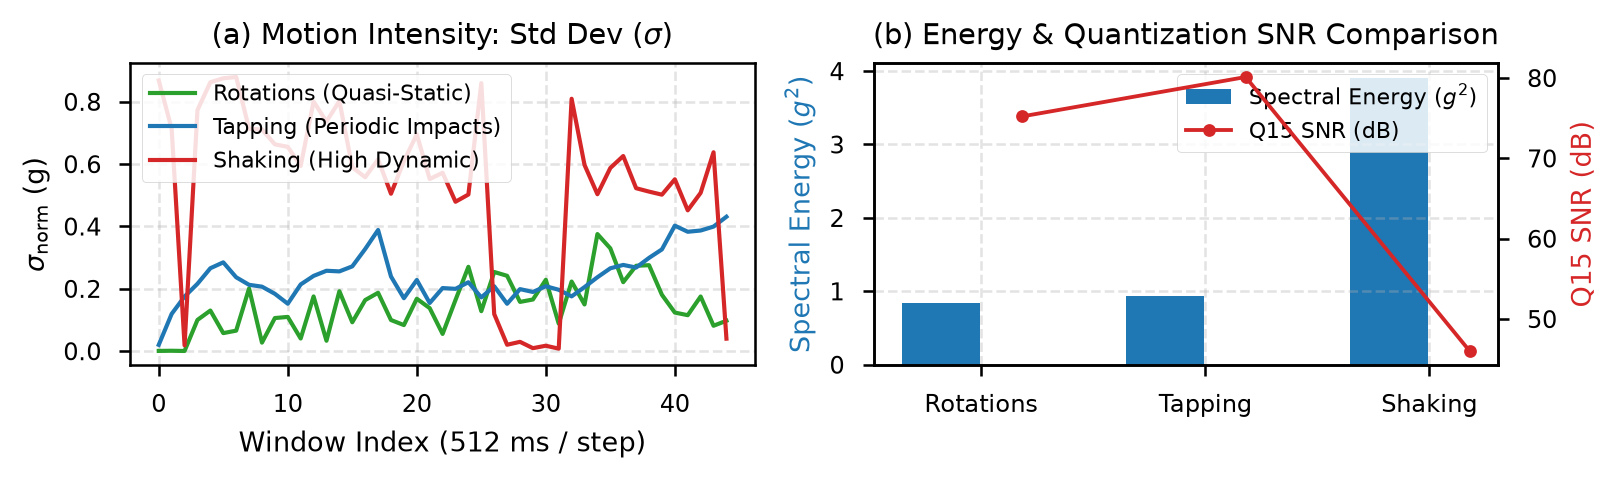
\includegraphics[width=\linewidth]{figures/fig_variations_overview.png}
    \vspace{-4mm}
    \caption{Comparative analysis across the three physical experiments: (a) motion intensity $\sigma$ over consecutive windows; (b) spectral energy and Q15 quantization SNR, demonstrating degradation under extreme dynamic shaking.}
    \label{fig:variations}
\end{figure}

\subsection{Quantization and Storage Benefits}
Quantizing processed windows to Q15 reduced sample storage from 4 bytes (\texttt{float32}) to 2 bytes (\texttt{int16\_t}) per sample, achieving an exact 2.0$\times$ reduction in SD card write bandwidth (from $6.0\text{ kB/s}$ to $3.0\text{ kB/s}$). Under normal motions (rotations and tapping), SNR remained high ($>75\text{ dB}$). During violent shaking, SNR decreased to $46.0\text{ dB}$ (Fig.~\ref{fig:variations}(b)) because peak acceleration transiently exceeded the normalized $\pm 2g$ threshold.

\section{Discussion, Issues, and Alternatives}

\subsection{Engineering Issues and Mitigations}
During hardware integration, two main challenges emerged:
\begin{enumerate}
    \item \textbf{SD Card Flushing Latency:} FATFS file sync operations occasionally incur 5--20~ms multi-sector write latencies. The dual-core decoupled producer-consumer design with a 512-sample FIFO queue entirely prevented buffer overflows.
    \item \textbf{Dynamic Acceleration vs. Sensor Range:} Shaking produced peaks up to $3.46g$, reaching sensor saturation on $\pm 2g$ scale. Increasing the full-scale range to $\pm 8g$ or $\pm 16g$ in software would resolve clipping during intense gestures.
\end{enumerate}

\subsection{Alternative Approaches and Future Enhancements}
While the current implementation achieves high fidelity and real-time responsiveness, several alternative designs could be explored:
\begin{itemize}
    \item \textbf{Sliding Overlapping Windows:} Replacing disjoint block windows with 50\% overlapping windows (hop size $H=128$) would double event detection rate and alleviate attenuation of impacts occurring at Hamming window boundaries.
    \item \textbf{CMSIS-DSP Fixed-Point Acceleration:} Utilizing Arm CMSIS-DSP integer FFT instructions (\texttt{arm\_rfft\_q15}) could leverage the RP2350 Cortex-M33 DSP extensions to reduce execution cycles by an estimated 65\%.
    \item \textbf{Integration with TinyML Classifiers:} The computed feature vector serves as an optimal input layer for a shallow Neural Network or Random Forest (as in Lab 2) to classify activities (e.g. idle vs. walking vs. shaking) on-device.
\end{itemize}

\section{Conclusion}
This work successfully implemented, compiled, and verified an embedded feature extraction and signal processing framework for IMU data on the Raspberry Pi Pico 2 W. By utilizing a dual-core architecture, the system guarantees jitter-free 500~Hz data acquisition alongside comprehensive time-domain statistical extraction, Hamming-windowed FFT peak detection, and Q15 quantization. Experimental validation across three physical activities confirmed exact numerical parity with PC reference models, $>75$~dB quantization SNR under normal motion, and a 2$\times$ storage reduction. The modular design provides an extensible foundation for on-device TinyML classification on resource-constrained embedded platforms.

\begin{thebibliography}{00}
\bibitem{dopico2020} D.~Dopico, D.~Luaces, F.~Gonzalez, and M.~Cuadrado, ``Dealing with real-time constraints in embedded sensor processing,'' \emph{IEEE Trans. Ind. Electron.}, vol.~67, no.~7, pp.~5921--5930, Jul. 2020.
\bibitem{oppenheim2009} A.~V.~Oppenheim and R.~W.~Schafer, \emph{Discrete-Time Signal Processing}, 3rd~ed. Upper Saddle River, NJ: Prentice Hall, 2009.
\bibitem{raspberrypi2024} Raspberry Pi Ltd., \emph{RP2350 Datasheet: High-performance microcontroller}, Cambridge, UK, 2024.
\bibitem{invensense2017} TDK InvenSense, \emph{ICM-20948 Automotive 9-Axis MotionTracking Device Datasheet}, San Jose, CA, 2017.
\end{thebibliography}

\end{document}
